%!TEX root = ../dissertation.tex

\chapter{Background}
\label{chapter:background}
In order to develop a programming environment for \gls{gd} that works in the cloud, we first need to study the current solutions.

Not all presented solutions are used exclusively for \gls{gd}.
\gls{gd} encompasses both 3D modeling and programming, so it makes sense to look at systems where at least one of these aspects is explored.
Furthermore, the solutions that are presented include both desktop-based and cloud-based applications to allow for an understanding of what is currently possible in the cloud and how it compares to what is available on the desktop.

For each of the application that will be described, we have to state clearly its nature, that is:
\begin{itemize}
	\item Is it a desktop-based or cloud-based application?
	\item Is it a programming environment? If so, what is its target audience?
\end{itemize}


%##############################################################################
%##############################################################################
\section{Related Work}


\subsection{Impromptu}
\label{section:impromptu:related}
Impromptu\cite{sorensen2005impromptu,sorensen2010programming} is a programming environment developed to explore manipulation of musical structure in live performance; an \gls{ide} for musicians and sound artists.

%What is live-performance?
Using Impromptu, live performance takes place as a musician programs algorithms that produce music in front of an audience.
During his performance, he writes the program that produces the sounds and chooses the right moments to change it to move between different parts of the music.

%What does it provide to support live-performance?
To enable live programming Impromptu brings together four components: an audio synthesizer, a real-time scheduling engine, a Scheme interpreter and an \gls{ide}\cite{sorensen2005impromptu}.
The first three components make up the runtime environment, responsible for producing the sound, while the last provides an user interface, where the musician writes code and sends it to the runtime in much the same way as using a \gls{repl}.

%Describe live programming experience of impromptu.
As he sends code, the musician builds the algorithm that produces the music incrementally.%
\footnote{The code sent to the runtime can define/redefine functions or variables, and schedule audio or functions to be played or run later.}
To be able to keep producing sound for the audience he can program simple patterns, send them to the runtime and then change them as he programs more elements to compose the music.
As he adds more elements he can start to make small changes to some of them which will be immediately audible.

The immediacy from program changes to audible ones also lets the musician experiment with new ideas.
Similarly, someone doing \gls{gd} will also benefit from having this immediacy in his \gls{ide}.

The separation of components referred earlier also allows several musicians to collaborate at the same time in a performance\cite{sorensen2005impromptu}.
Each one using a computer connected to the same runtime environment, they can build different parts of the music or, more interestingly, make changes to parts of the other's work.
This is also an interesting aspect to explore in architecture, where several architects can work on a \gls{gd} program at the same time, each one showing his ideas on how to evolve the design.

There is, however, a major difference between composing music and architecture.
As sound is an ephemeral phenomenon, music's complexity comes from how sounds are organized in time as opposed to architecture's complexity, which comes from how shapes are organized in space.
The point is, music/sound generation is a continuous process whilst architecture/form generation is a instantaneous process.
\begin{description}
	\item[Music] produce samples at 44kHz
	\item[Architecture] produce model of 100k shapes + display model of 100k shapes at 25+Hz
\end{description}
There are differences in performance that will affect the architecture of the system and its usage experience.


\subsection{LightTable}
\label{lighttable:related}
LightTable\cite{lighttable2015site} is a code editor for the Clojure programming language\cite{hickey2008clojure} and is an example of a desktop application that uses web technologies.
More specifically, it uses nw.js\footnote{nwjs.io} as its runtime allowing it to use the html layout engine for its user interface, to use Javascript as its programming language and to use node.js\cite{tilkov2010node} modules.
LightTable is written in ClojureScript\cite{10.1109/MIC.2011.148}, a subset of Clojure that compiles to Javascript.

Although not related to \gls{gd}, LightTable as proposed some interesting features and concepts for \glspl{ide}.

%Why is LightTable relevant?
One of these is the use of the drafting table as metaphor.%
\footnote{http://www.chris-granger.com/2012/04/12/light-table-a-new-ide-concept/}
The metaphor comes from looking at the way work is done in other fields of engineering, where engineers spread all materials relevant to their work over large tables, from tools to reference information.
Instead of displaying the contents of entire files, LightTable divides the code into meaningful units and displays them as small editors spread over the table's surface.
In one of its experimental versions, LightTable also supported displaying running programs in the table.
Fig. \ref{fig:lt:draft:table} shows an example of this metaphor, which has some resemblance to node-based programming environments.
The programmer still has to think of how to arrange what is on the table.
What makes it different is allowing to choose what is on the table instead of having everything on it all the time.

\begin{figure}
  \centering
  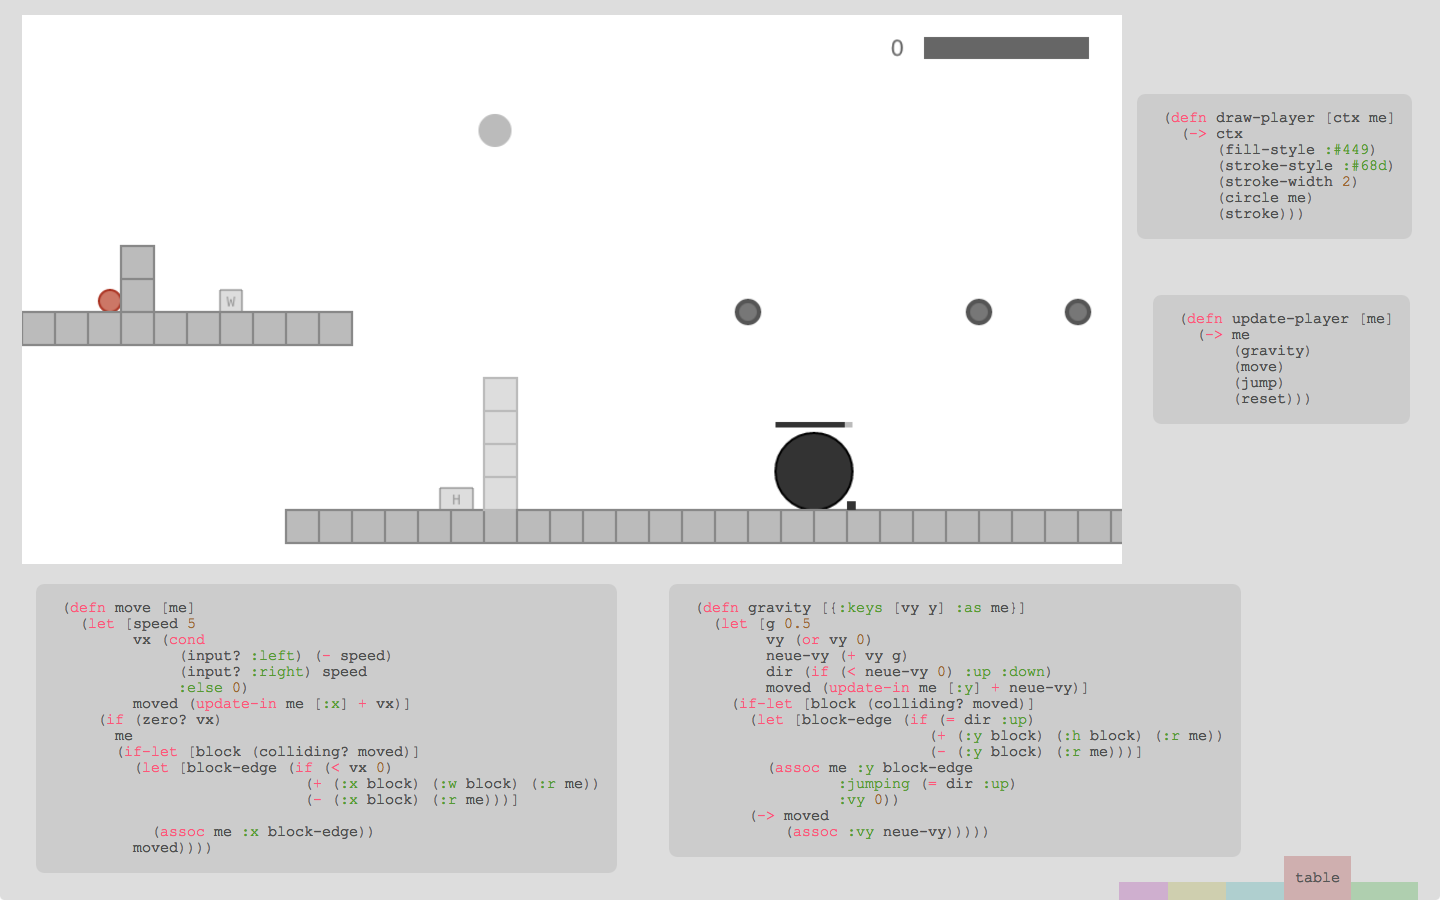
\includegraphics[width=12cm]{./images/lt_game_example__inv}
  \caption[LightTable's drafting table showing a game.]{LightTable's drafting table. A game is being run inside it while some of its code is displayed in separate editors.}
  \label{fig:lt:draft:table}
\end{figure}

%LightTable "function navigation"
Other feature deals with how to help navigating Clojure code bases.
In Clojure, functions are defined inside namespaces and all Clojure definitions (functions, variables, macros) are stored in text files.
Navigating among definitions and the current namespace structure should not get in the way of editing code.
To make editing easier, LightTable provides a \emph{namespace browser} that allows to find functions and a \emph{code document} where functions can be added for editing without moving them out of their namespace or displaying entire files where they are defined.
Fig. \ref{fig:lt:clojure:table} shows an experiment where these two are used.

\begin{figure}
  \centering
  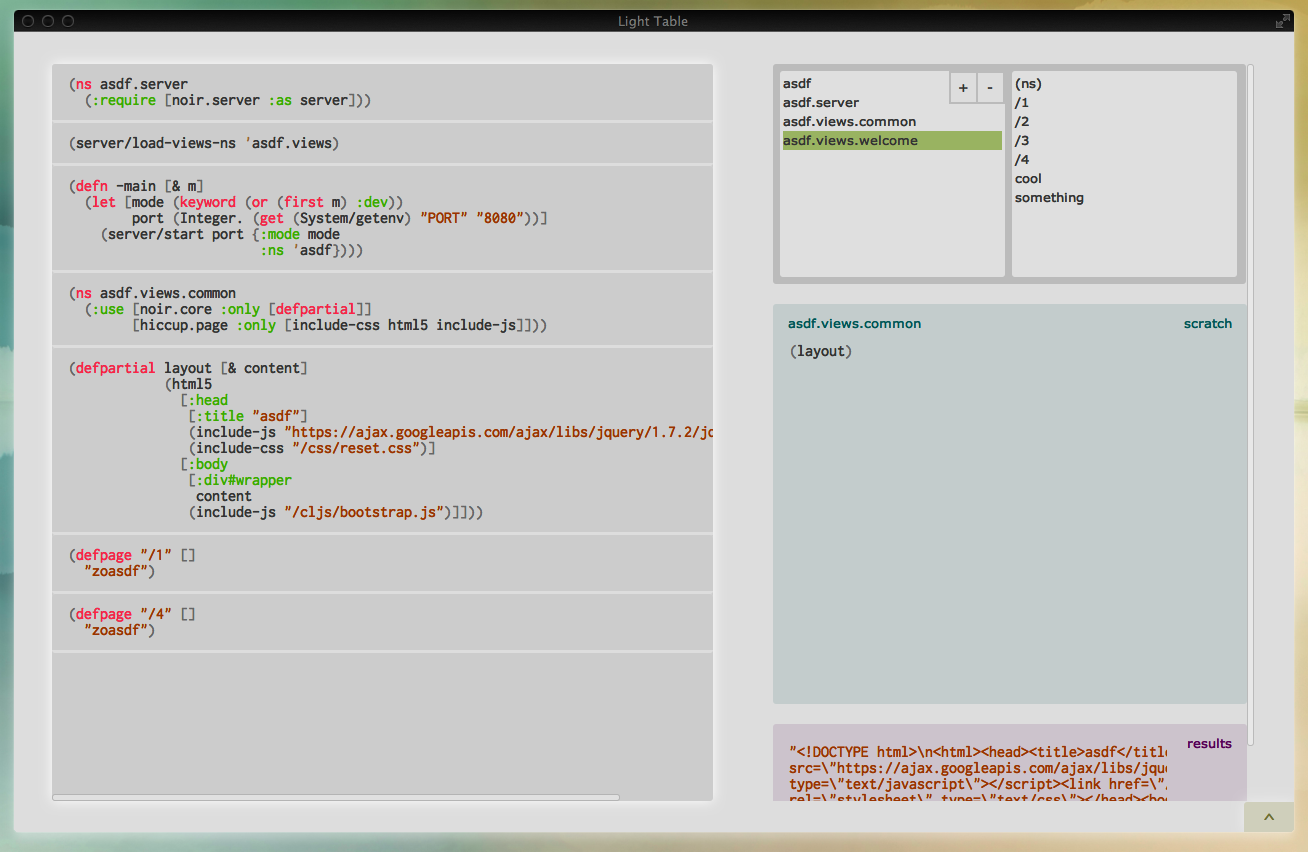
\includegraphics[width=12cm]{./images/lt_clojure_table__inv}
  \caption{An experiment showing a \emph{code document} on the left and a \emph{namespace browser} on the top right.}
  \label{fig:lt:clojure:table}
\end{figure}

%LightTable "variable substitution"
Another interesting feature of LightTable is its ability to show data flow in a function call.
Since the main purpose of a function is to transform its input data into its output data, it helps to see what happens to the data on each step of the function.
To achieve this, LightTable overlays variable values and return values, respectively, on each variable occurrence and expression of the function.
Fig. \ref{fig:lt:val:overlay} shows an example of such functionality.
This functionality is part of LightTable's \emph{instarepl}.

This last feature has the problem of not being capable of showing the data-flow for more than one run of a part of the code.
If a function is called more than once then it will be more useful to show the data-flow of all the calls.

\begin{figure}
	\centering
	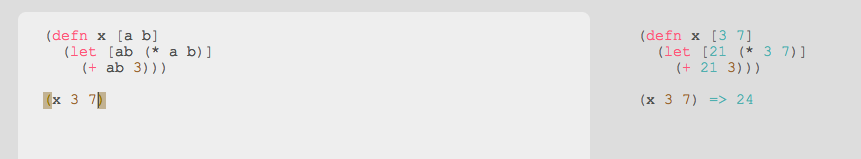
\includegraphics[width=12cm]{./images/lt_val_overlay__inv}
	\caption{An example of LightTable's value overlaying. The occurrences of the variables \emph{a}, \emph{b} and \emph{ab} were replaced with their values while evaluating the expression \emph{(x 3 7)}; the result of this expression is also overlaid.}
	\label{fig:lt:val:overlay}
\end{figure}

Finally, the way LightTable is structured is also relevant as it makes possible to modify its behavior at runtime.
The main design pattern used in LightTable is the \gls{bot} pattern.
As described by one of its developers,\footnote{http://www.chris-granger.com/2013/01/24/the-ide-as-data/ at Nov/2015.} LightTable can be described as a set of \emph{Objects}, each having a set of \emph{Behaviors} and being tagged with a set of \emph{Tags}.
The \emph{Behaviors} describe how an \emph{Object} reacts when events are raised on it. \emph{Tags} are groups of \emph{Behaviors}.
When an event is raised on an \emph{Object} both its \emph{Behaviors} and those from its \emph{Tags} are notified.


\subsection{IPython}
\label{section:ipython:related}
IPython\cite{PER-GRA:2007} is a notepad-like environment (Fig. \ref{fig:ipython:notebook}) directed towards providing better, more straightforward, scientific computing.

As its name suggests, IPython's main programming language is Python.
Nevertheless, other popular programming languages can be used in IPython, particularly those popular in the scientific community like R, or Julia.%
\footnote{More language kernels can be found in IPython's github page: https://github.com/ipython/ipython/wiki/IPython-kernels-for-other-languages}

One trend in its community, one that is supported by IPython notebooks, is to make results in publications more reproducible.
Typically, the code used to compute the results showed in publications is not made available to the public, so it is harder for a stranger to check them.
Instead of publishing a PDF or making a blog post, authors write whole publications as IPython notebooks which then are shared and thus allow everyone to run their source code.
Having access to a working copy of the notebook, one can also experiment with it to better understand it, form own conclusions, and find potential errors.

%IPython architecture
IPython was decomposed into execution kernels, a communication protocol, and several front-ends.
Execution kernels are responsible for running the code of notebooks and front-ends implement the \gls{ui}, as is the case of IPython's notebooks.
The communication protocol defines how communication between execution kernels and front-ends is done.
With this, it is possible to implement new execution kernels for running code from a programming language not yet implemented or an alternative front-end different from IPython notebooks.
Moreover, the communication protocol also allows execution kernels and front-ends to run on different computers\cite{PER-GRA:2007}.

\begin{figure}
	\centering
	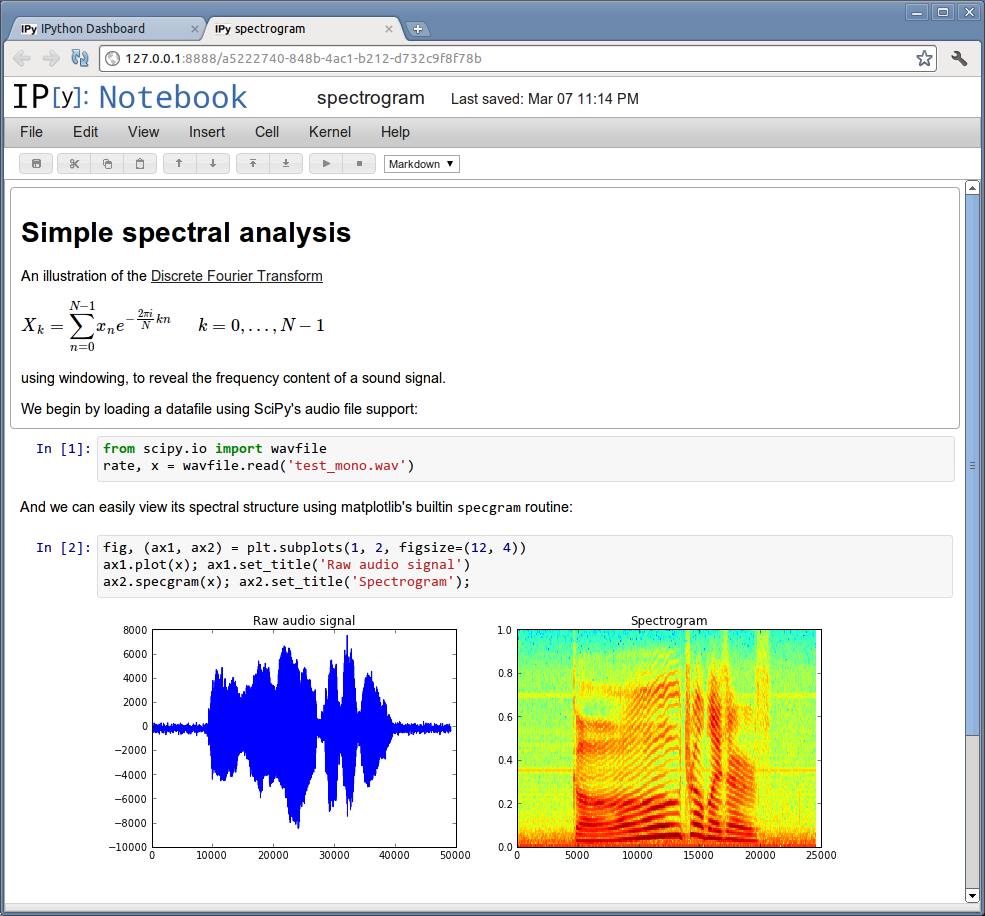
\includegraphics[width=0.8\textwidth]{images/ipython_notebook}
	\caption{An IPython notebook with rich text, mathematical notation, source code and results from executing such code.}
	\label{fig:ipython:notebook}
\end{figure}

%Why is it important? I cannot imagine designers using it.
As seen in Figure~\ref{fig:ipython:notebook}, IPython's notebooks can contain not only source code but also its results and rich text.
The style of producing notebooks in IPython is one that mixes programming, writing and exploring.
Interestingly, this style is also part of a designer's processes.
Like a scientist, the designer also has to do exploration of ideas (design ideas in his case), reach conclusions (finished designs) and share his work with others (fellow designers, clients, friends, blog readers).
Unfortunately, although IPython notebooks are natural tools for exploration, they do not provide domain specific functionality for architecture.


\subsection{OpenJSCAD}
OpenJSCAD\cite{openjscad2015site} is a project aiming to implement OpenSCAD\cite{kintel2011openscad} using web technologies.
Instead of using OpenSCAD's language, OpenJSCAD uses JavaScript as its language.
Most of OpenSCAD functionality is implemented in OpenJSCAD.
Like OpenSCAD, it focuses on creating 3D models for 3D printing.

Similarly to the \gls{gd} approach, to actually model in OpenJSCAD the user has to write a program in either Javascript or OpenSCAD's language.

Being an environment for modeling 3D printed objects, OpenJSCAD supports importing and exporting 3D models from/to STL and AMF files which are commonly used as 3D printing formats.

OpenJSCAD provides two user interfaces, one command-line interface and one graphical user interface as a web page.%
\footnote{https://github.com/Spiritdude/OpenJSCAD.org}
The first can be used for batch processing, while the second integrates an editor to edit a program and a 3D view for viewing the results of that program.
This separation enables the use of OpenJSCAD for programming without requiring the programmer to install anything more than a web browser, which is almost always already installed.
This is just a matter of convenience, since both interfaces perform the same work to generate the models and both can export them as files.

OpenJSCAD makes its functionality available as functions as well as methods on its objects, which makes writing programs more flexible.
This way, one can write either \mintinline{javascript}{a.union(b).translate([1,0,3])}, \mintinline{javascript}{translate(union(a,b), [1,0,3])} or \mintinline{javascript}{union(a,b).translate([1,0,3])} depending on what is more readable.%
\footnote{The first can be read as \emph{a united with b, translated by [1,0,3]}, the second as \emph{the translation of the union of a and b by [1,0,3]} and the third as \emph{the union of a and b, translated by [1,0,3]}.}

Both OpenJSCAD's functions and methods return new objects and do not have side-effects.
This allows the programmer to use the functional programming paradigm and makes it easier to understand programs, as there are less side-effects that could change their behavior.

A problem that can arise while writing and testing JSCAD programs is that there is no help on getting the parameters for operations right and it is frustrating to spend more time than acceptable trying to understand why a certain operation is not producing the desired result.
This problem is even more relevant when most of the operations have multiple optional parameters and there are parameters that replace other parameters.
Currently, the only help available is OpenJSCAD's documentation (a tour on its functionality), the online community around OpenJSCAD and, since Javascript is its language, web browsers' Javascript developer tools.


\subsection{Processing}
\label{section:processing:related}
Processing\cite{reas2007processing} is a programming language and a development environment aimed at ``promoting software literacy in the visual arts and visual literacy within technology''.%
\footnote{Quoting www.processing.org, 9/Nov/2015.}
It is a desktop application.

Processing enables everyone to write programs that both draw to the screen and react to input from the user, like moving the mouse or pressing a key on the keyboard.
It makes this possible by implementing most of the functionality that is commonly required, like initializing the drawing surface, so the programmer only has to implement the functionality specific to the result he wants to achieve.
The code in Listing \ref{lst:simple:processing}, for instance, is what is needed to setup a drawing canvas, its background color and continuously draw a line from the mouse position to a point on the canvas.

To use Processing's programming language, one needs to use its \gls{ide}, the \acrfull{pde}.
As shown in Fig. \ref{fig:proc:dev:env}, the \gls{pde} includes a text editor with syntax highlighting and runs Processing programs.

\begin{listing}
\begin{minted}[linenos,frame=lines]{java}
//Hello mouse.
void setup() {
	size(400, 400);
	stroke(255);
	background(192, 64, 0);
}

void draw() {
	line(150, 25, mouseX, mouseY);
}
\end{minted}
	\caption[A simple Processing sketch]{A simple Processing sketch}
	\label{lst:simple:processing}
\end{listing}

\begin{figure}
	\centering
	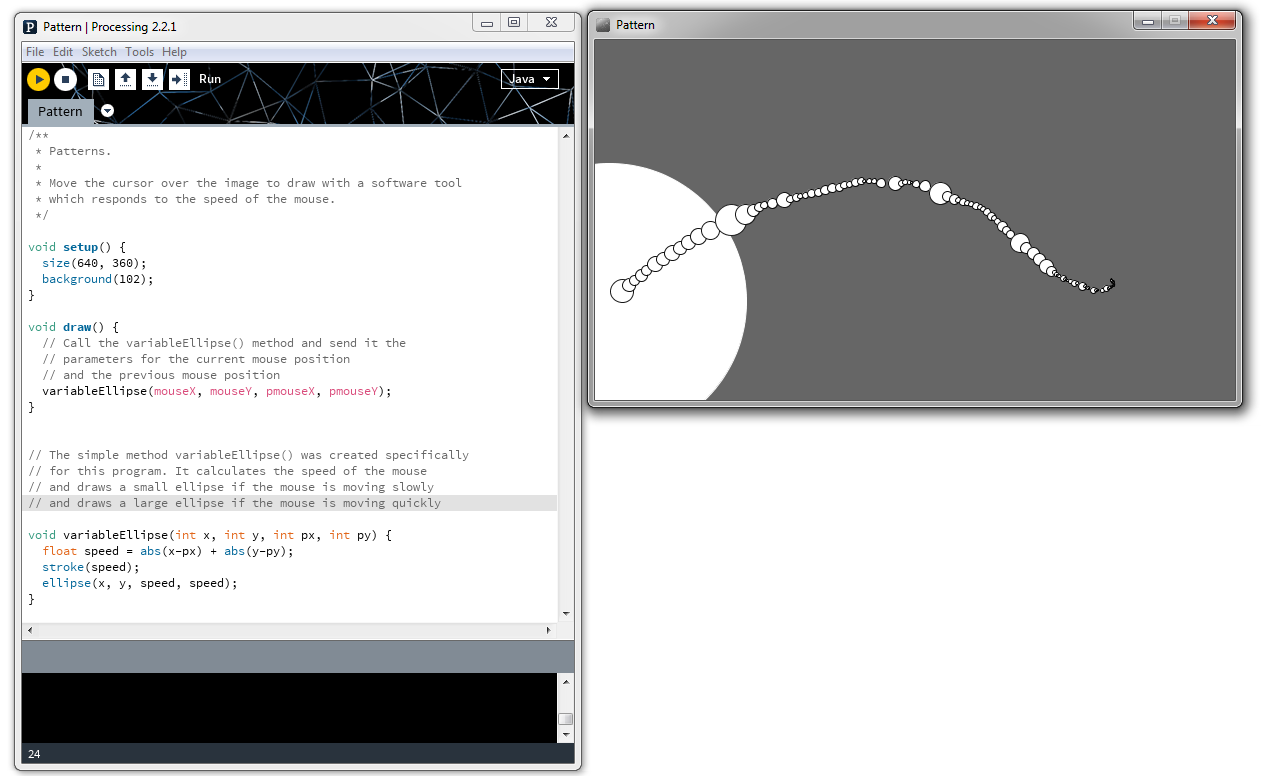
\includegraphics[width=1.0\textwidth]{images/proc_dev_env}
	\caption{On the left: The \gls{pde} displaying an example \emph{sketch} while it is being run. On the right: The drawing window to which the \emph{sketch's} instructions are applied.}
	\label{fig:proc:dev:env}
\end{figure}

Processing is sometimes used by architects for exploring design ideas.
However, since most of its functionality revolves around graphics for the visual arts, its use is normally restricted to 2D designs and cannot be used as a full-fledged tool for \gls{gd}.


\subsection{DesignScript}
\label{section:designscript:related}
DesignScript\cite{aish2012designscript} is a programming language that was designed to suit the needs of architecture related design.

%DesignScript programming paradigms
DesignScript uses concepts from multiple programming paradigms like object-oriented, functional and associative programming.
Entities have properties that can be either data or functions like in object-oriented languages; functions' most important role is to take some input and produce some output without producing side-effects like in functional languages; and dependencies among variables are retained like in associative languages.

It supports both imperative (following instructions step-by-step) and associative (propagating changes in a dependency graph) control flows.
The programmer can choose to have portions of the code following one type of control flow and other portions following the other.

%DesignScript primitives
Being a domain-specific language for architecture, DesignScript provides functions for 3D modeling such as creating concrete 3D objects, like cubes and spheres, as well as abstract geometry, like planes and points, that is used as scaffolding.

DesignScript also supports lists of values and lets them be used in place of single parameters in calls to functions.
This lets architects use lists more easily as they do not have to use loops to extract values and pass them to functions.%
\footnote{If only one of its parameters is receiving a list instead of a value, the function is called once with each value on the list.
If more than one parameter is receiving a list, the function is called with the values combined by either a cross product or a zip of the lists.}

Having modeling primitives and combining several programming paradigms allows the architect to draw from knowledge about architecture modeling while empowering him to express the processes in which those primitives are used.

%DesignScript editor(s)
Editing DesignScript programs can be done either by writing or by creating a graph.
The graph is a more natural representation of the dependencies between the variables of the program when the associative paradigm is being used; it can also be viewed as a data-flow graph.
The written representation of DesignScript is a sequence of statements that specify the relationship between a variable and other variables; defining functions, using the imperative paradigm and reassigning variables is also possible.

DesignScript is used in several environments, all of which are desktop applications.
These include a textual editor in Autodesk AutoCAD (Fig. \ref{fig:ds:autocad}), a dedicated graph editor called DesignScript Studio (Fig. \ref{fig:ds:dsstudio}) and later Dynamo (Fig. \ref{fig:ds:dynamo}).
Both DesignScript Studio and Dynamo use graph based program editing.

\begin{figure}
	\centering
	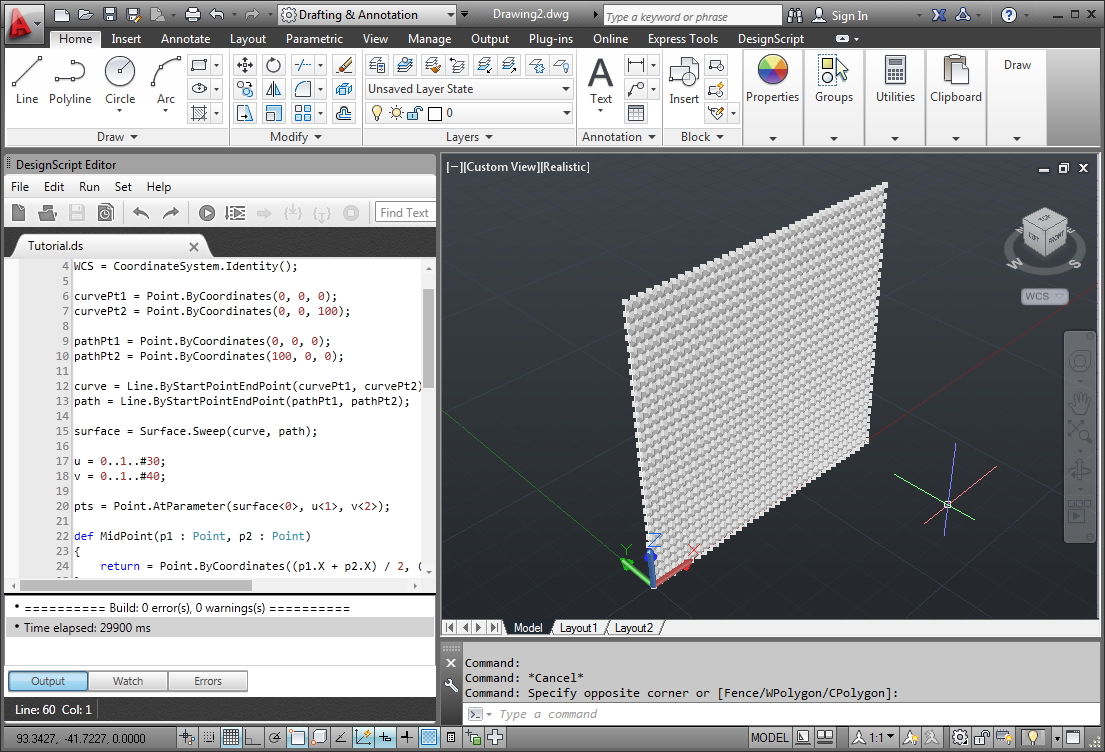
\includegraphics[width=0.8\textwidth]{images/ds_autocad}
	\caption{A DesignScript program being edited in a special text editor inside AutoCAD. This text editor provides auto-complete and a debugger.}
	\label{fig:ds:autocad}
\end{figure}

\begin{figure}
	\centering
	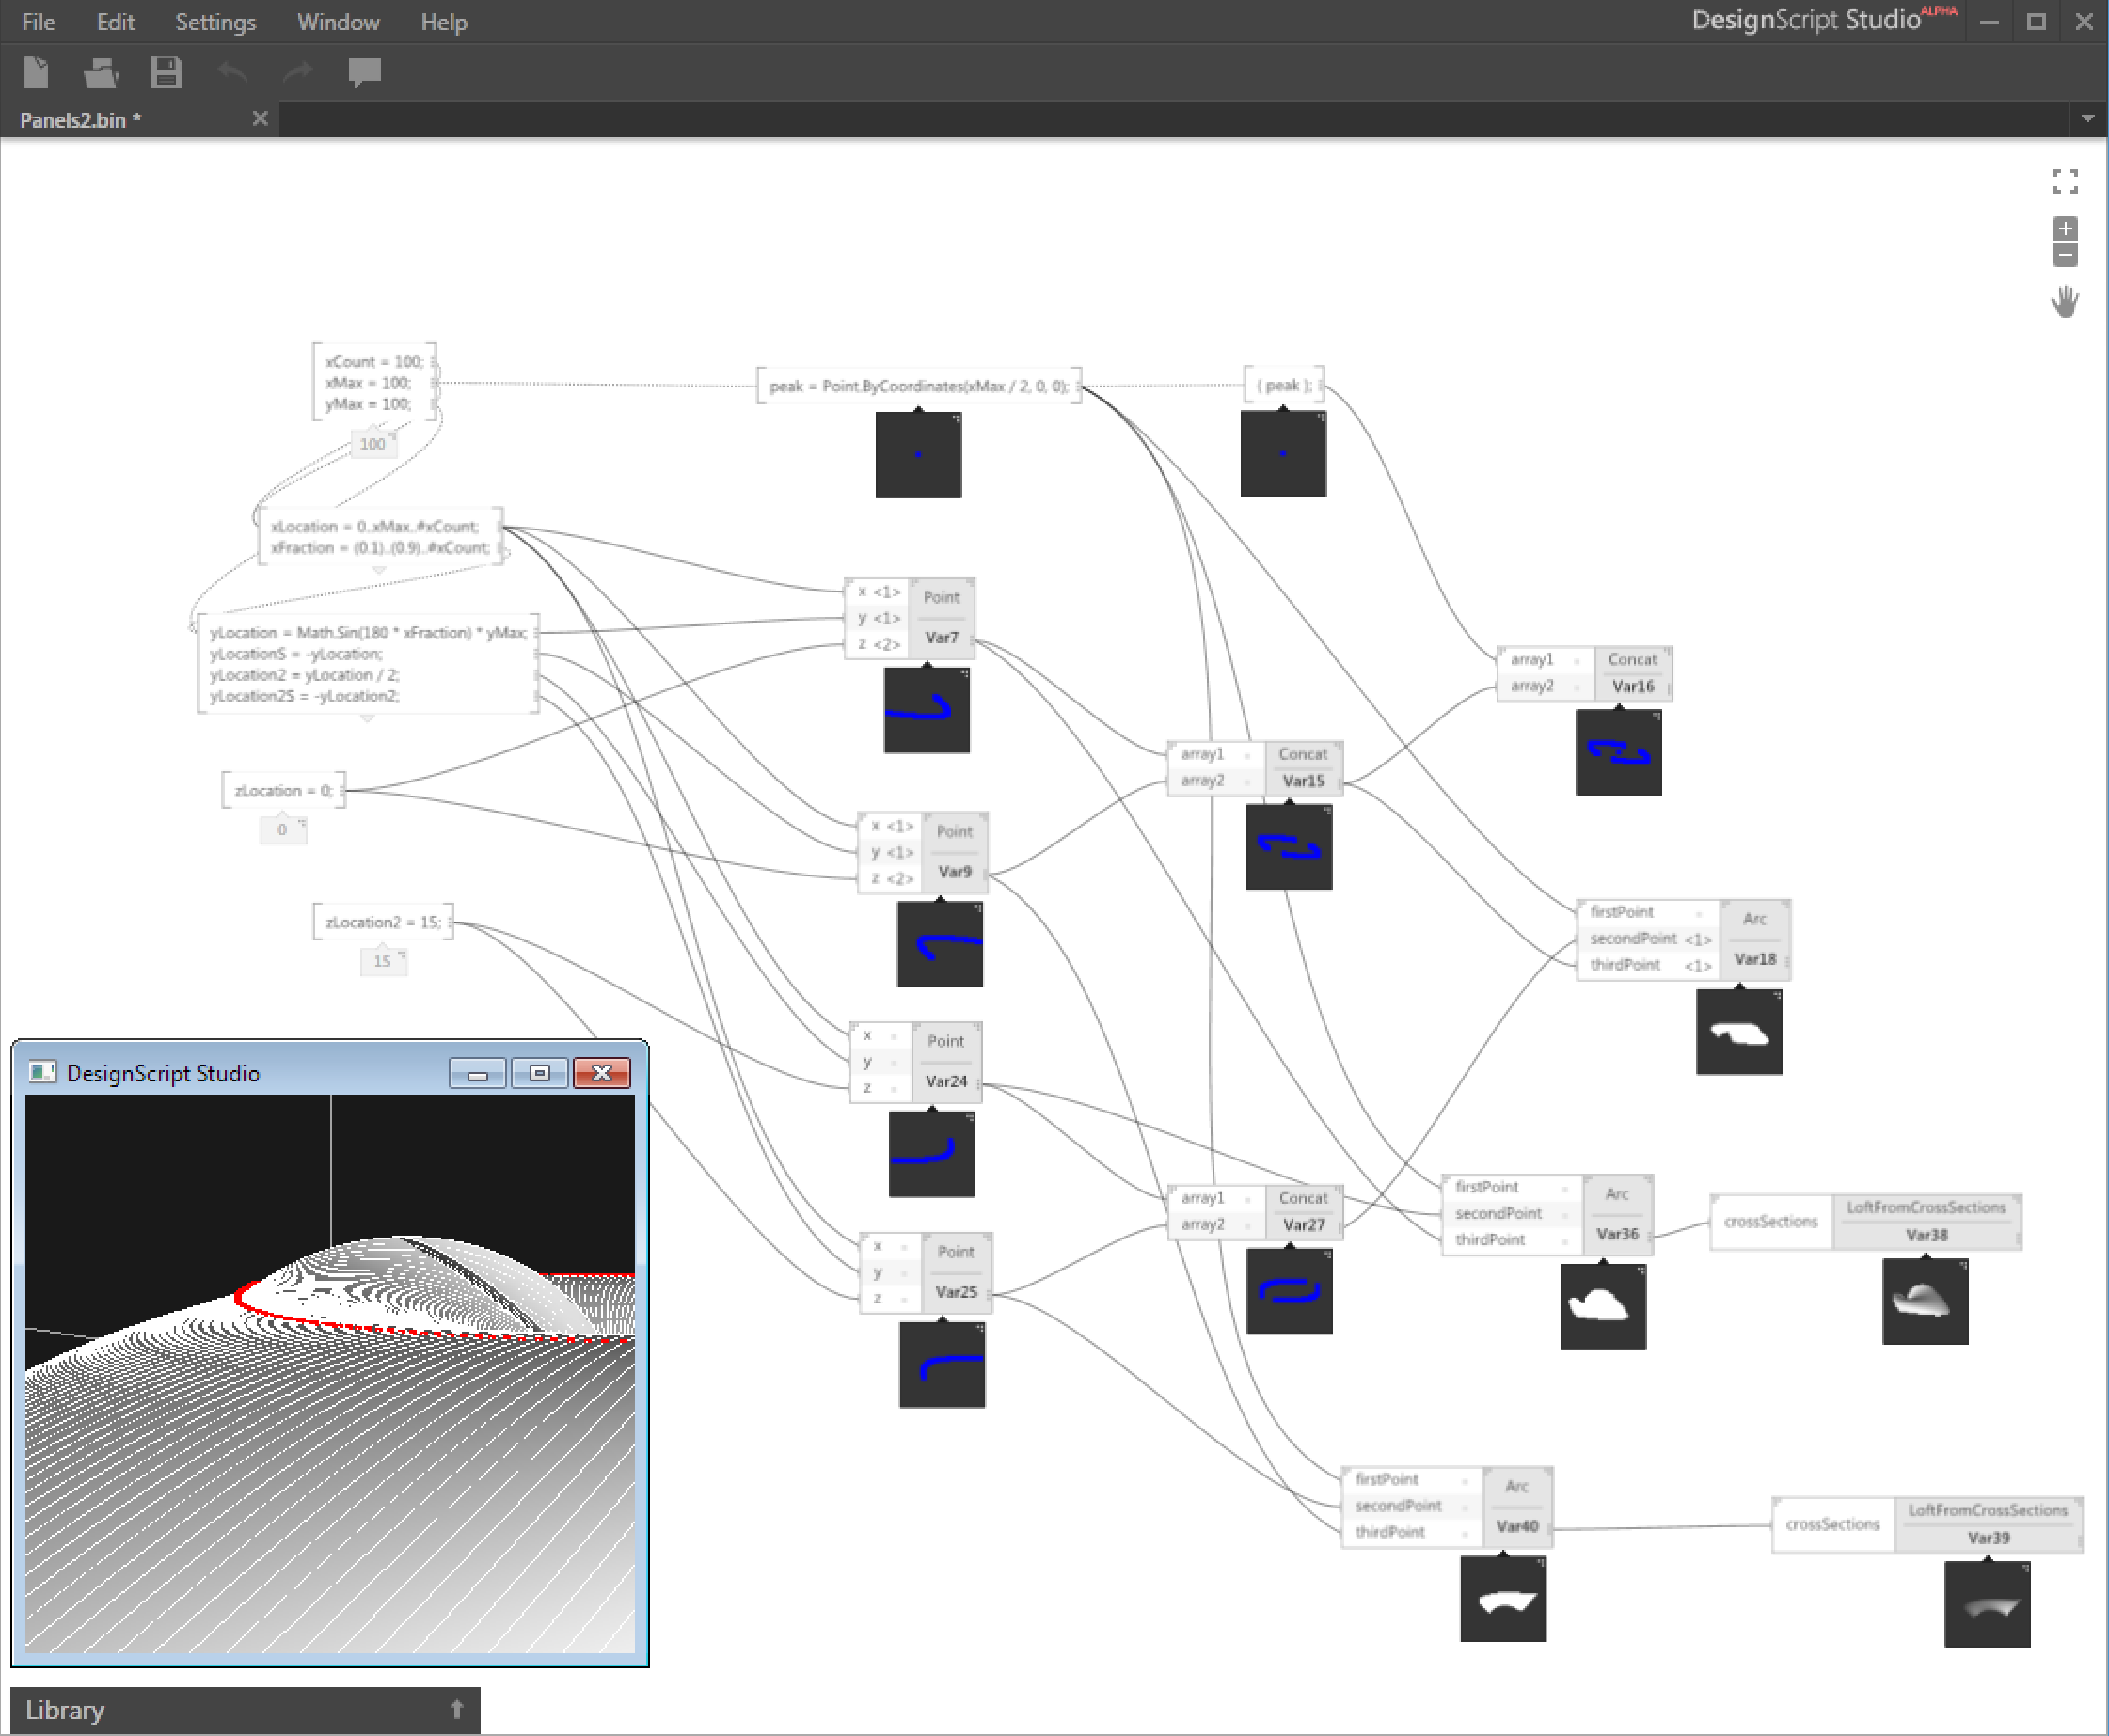
\includegraphics[width=0.8\textwidth]{images/ds_dsstudio}
	\caption{A DesignScript program as a graph in DesignScript Studio. Each node can display a preview of its results. To the bottom left corner is a preview of the whole program results and a folded library tab. The library tab contains everything that can be used in the program.}
	\label{fig:ds:dsstudio}
\end{figure}

\begin{figure}
	\centering
	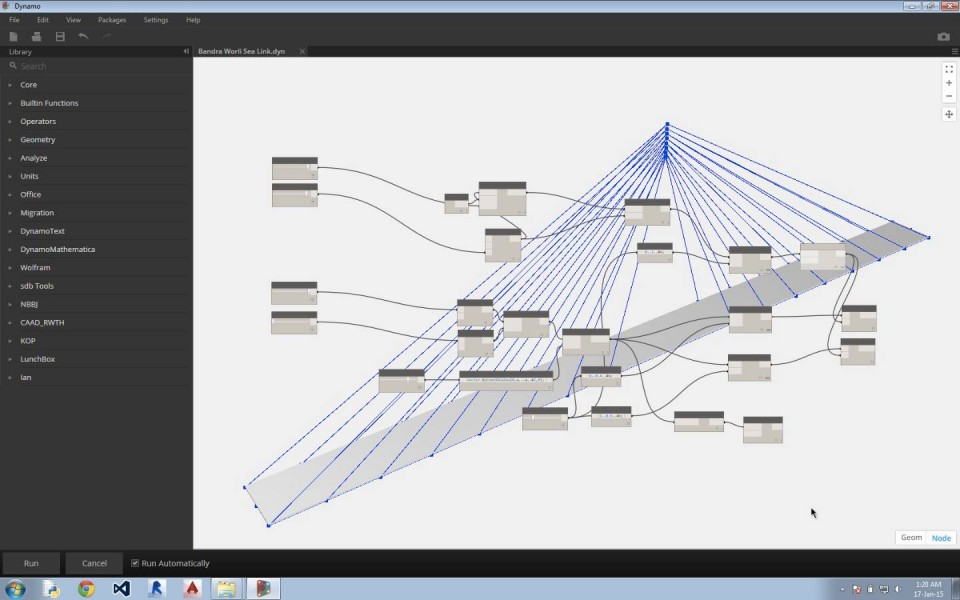
\includegraphics[width=0.8\textwidth]{images/ds_dynamo}
	\caption{Another DesignScript program as a graph in Dynamo. Like in DesignScript Studio, a preview of the result of the program is displayed. A difference is that there is only one preview ``canvas''; the preview from selected nodes is highlighted.}
	\label{fig:ds:dynamo}
\end{figure}

Debugging DesignScript programs depends on the environment being used.
The textual environment allows to follow the execution of the program step-by-step while also supporting watches and breakpoints.
The graph-based environments allow highlighting and listing results of each node.
Both the textual and the graph-based environments provide a preview of the execution of programs.

%DesignScript history
DesignScript was later used as the scripting language for code blocks in Dynamo\footnote{http://dynamoprimer.com/}, integrated with Autodesk Revit, where programs are edited as data-flow graphs.
DesignScript was also integrated into Autodesk AutoCAD.
A standalone node-based DesignScript editor was also made, it was called DesignScript Studio.


\subsection{Rosetta}
\label{section:rosetta:related}
Rosetta\cite{de2012modern,lopes2011portable}, shown in Fig. \ref{fig:rosetta:ex}, is an environment for \gls{gd}.

Most CADs architects use allow them to make \gls{gd} programs.
The problem with programming is that as each of these CADs has specific primitive operations, so, programs written for one CAD will only work in that CAD.
A phenomenon called vendor lock-in.
As an example, if one writes a program for AutoCAD, he cannot use it in Rhinoceros3D.
If he really wants to use it in Rhinoceros3D, he has to rewrite it taking into account the differences between primitive operations of both \glspl{cad}.

Rosetta's motivation is to allow architects to write portable \gls{gd} programs that generate equivalent models in any CADs they use.

Rosetta does this by allowing the architect to choose the front-end programming language and the back-end where the primitive operations will be performed.%
\footnote{Some front-ends supported by Rosetta are AutoLisp (one of AutoCAD's programming languages), Javascript, Racket and Python; some of the supported back-ends include CADs like Autodesk AutoCAD, Autodesk Revit, Sketchup, and Rhinoceros 3D and also graphics libraries like TikZ and OpenGL.}
This way, the architect can experiment with \gls{gd} without having to switch \gls{cad} and he can also share programs with others using different \glspl{cad}.

Rosetta also allows programs written in one programming language to use not only parts from programs written in the same language, but also from programs written in other languages.
This eliminates the need to use the same programming language throughout a program and enables the use of programs written in any programming languages.

\begin{figure}
	\centering
	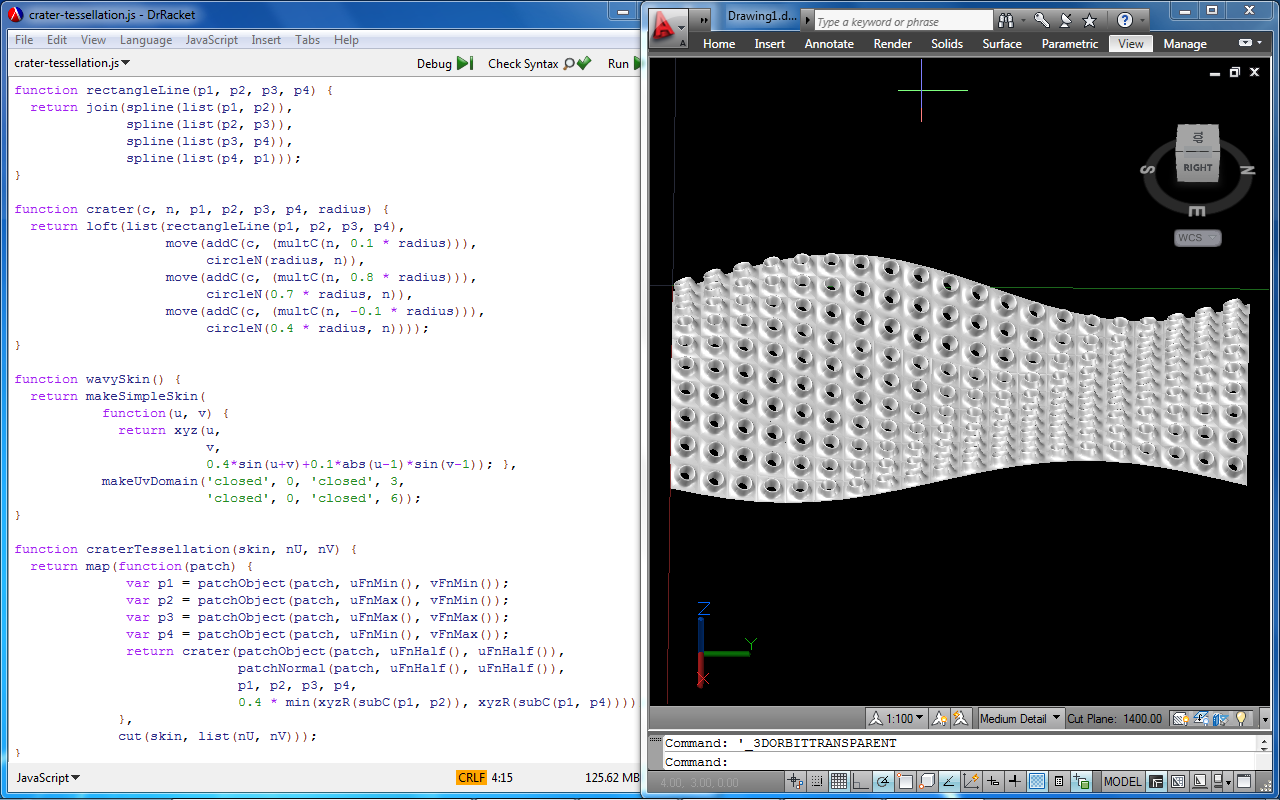
\includegraphics[width=0.8\textwidth]{images/rosetta_js_autocad}
	\caption{A Rosetta program (left) and AutoCAD displaying its results (right). The program is written in Javascript.}
	\label{fig:rosetta:ex}
\end{figure}


\subsection{Clara.io}
Clara.io is a web application for 3D modeling like Blender and 3ds Max.
It is thought as a tool for 3D modeling people (3d artists, architects).
The modeling process is mainly done using direct manipulation.
Uses WebGL for 3d view and has integration with VRay cloud rendering.
Its scenes are stored remotely, so it does not matter which computer is being used.
Scenes can be edited by several people with real-time collaboration.

It does have scripting support but it serves as an automation tool for the direct manipulation process.
It is intended to be used as an \gls{api} for plug-in development.%
\footnote{https://clara.io/learn/sdk/scripting}


\subsection{OnShape}
OnShape\footnote{https://www.onshape.com/} is a cloud based \gls{cad} application.
Unlike Clara.io, OnShape is aimed at product design and, as such, its users are familiar with 3D modeling software like SolidWorks and Autodesk Inventor.

Like most cloud applications, it promotes collaboration on development teams where team members work remotely.
In order to do this, OnShape makes it possible for multiple users to edit the same files.
It has version control of project documents (drawings, 3d models, text documents) and supports real time collaboration.

Supposedly, it can be accessed using web browsers and also mobile devices.

\begin{description}
	\item[collaboration] control access rights, simultaneously on the same branch of a document, or independently on different branches which can be merged later (some or all changes)
	\item[data management] everything is recorded, undo stacks per tab, document history (branch history)
\end{description}

OnShape also includes a dedicated programming language, FeatureScript, for defining features for its models.
OnShape includes an \gls{ide} for FeatureScript but the language does not aim to replace OnShape's modeling approach based on a feature list.


\subsection{Mobius}
Prototype
Parametric modeling? Block based programming + Visual programming? 3D modeling?

Mobius combines block-based programming and visual programming as a way to make it more intuitive for architects to build programs.
In Mobius, programs are a combination of nodes in a data-flow graph that ultimately produces a 3D model.

The user can implement custom nodes by literally building a program out of virtual building blocks.
Each node is implemented as an imperative procedure.
This way, Mobius tries to get the best of visual and textual programming languages.

The block based approach has been used in pedagogical programming environments and seems to be most suitable for building procedural programs.


\subsection{RepoCad}
Prototype
2D drawing? Integrated version control? Sharing library?
Where is the juice???


\subsection{Antimony}
Refs: matt keeter thesis + blog
Handles UI? Design to fabrication pipeline? Visual programming? Distance field representation? Mac + Linux?

Antimony is a solid modeling tool where the user uses a visual programming language to define the models.
Like with other visual programming environments, programs come into existence by connecting nodes together.
Antimony also displays handles in the 3D view that can be dragged with the mouse to change properties of some nodes of the program being edited.

Antimony was implemented as a tool to be used from design to fabrication, so it can generate files for machining or 3D printing its models.

It is possible to implement custom nodes by writing a Python program with custom directives.
This program defines what are the inputs and outputs of the node and what is its \gls{ui} in the 3D view.
As Antimony uses \glspl{sdf} as its representation of solids, shapes are defined by specifying a formula for the shape's \gls{sdf} and its bounds.

%##############################################################################
%##############################################################################
\section{Comparison}

(app, desk/web/mobile, domain?, programming?, visual/text, primitives?, feedback?)\\
(app-cloud, storage?, collaboration?)\\
(app, ui-features/user-experience?)\\
app, domain, visual/text, desk/web/mobile,\\
app, storage, collaboration\\
3d functionality/geometric modeling/CAD capabilities\\

\begin{table}
	\centering
	\renewcommand{\arraystretch}{1.2}

	\begin{tabulary}{\textwidth}{r|L|L|L|}
									& {\bf Domain} 						& {\bf Programming} 															& {\bf Platform} \\
		\hline\hline
		Impromptu			& music, live coding			& textual(high+low level)													& desktop + local server					\\
		LightTable		& general coding					& textual, many languages													& desktop													\\
		IPython				& scientific computing		& textual, many languages													& web page + server(remote/local)	\\
		OpenJSCAD			& 3D CAD									& textual																					& web page, command-line					\\
		Processing		& visual arts							& textual																					& desktop													\\
		DesignScript	& CAD, architecture				& textual + visual																& desktop													\\
		Rosetta				& CAD, architecture				& textual, many languages													& desktop													\\
		Clara.io			& 3D modeling, animation	& limited(primarily for plug-ins and automation)	& cloud(web page)									\\
		OnShape				& 3D CAD									& textual(for custom model features)							& cloud(web page, mobile)					\\
		Mobius				& 3D CAD									& block-based + visual														& web page												\\
		RepoCad				& 2D CAD									& textual																					& web page/cloud									\\
		Antimony			& 3D CAD									& visual(main) + textual(custom nodes and shapes)	& desktop													\\
	\end{tabulary}
	\label{table:general:comp}
	\caption{General environment comparison}
\end{table}

\begin{table}
	\centering
	\renewcommand{\arraystretch}{1.2}

	\begin{tabulary}{\textwidth}{r|L|L|L|}
									& {\bf Storage} 						& {\bf Collaboration} 												& {\bf Coding features} \\
		\hline\hline
		Impromptu			& ---												& shared runtime															& sound changes; eval expression																						\\
		LightTable		& ---												& ---																					& instarepl; documentation; code completion; (code document); (draft table) \\
		IPython				& ---												& ---																					& code completion; different cell types																			\\
		OpenJSCAD			& ---												& ---																					& autorun; user-defined sliders																							\\
		Processing		& ---												& ---																					& syntax errors annotation;																									\\
		DesignScript	& ---												& ---																					& library tab; result highlighting																					\\
		Rosetta				& ---												& ---																					& user-defined sliders																											\\
		Clara.io			& cloud, version controlled	& share scenes, scene realtime collaboration	& ---																																				\\
		OnShape				& cloud, version controlled	& share documents, realtime collaboration			& --- ?																																			\\
		Mobius				& ---												& ---																					& sliders on node inputs																										\\
		RepoCad				& cloud, version controlled	& share scripts through library								& autorun																																		\\
		Antimony			& ---												& ---																					& autorun; 3D view handles																									\\
	\end{tabulary}
	\label{table:features:comp}
	\caption[Features / User experience comparison]{Features / User experience comparison. Collaboration on applications that do not support it is handled by users. }
\end{table}

Tables \ref{table:general:comp} and \ref{table:features:comp} allow us to compare these systems in terms of their domain, programming support, platform, storage, collaboration and coding features.

As can be observed, not all environments support \gls{gd} programming.
We want to look at cloud applications, programming environments and modeling/CAD environments.
It was also important to look at traditional 3D modeling environments and programming environments for domains where design is also present.


Although all environments have support for programming, the degree to which it was thought to be an alternative to the main activity is different.
Programming can be used in two ways: to be the way the user solves his problem; or, to extend the environment with more tools for the user.
Some of the analyzed environments support both ways while others only support one or the other.
To solve: Impromptu, IPython, OpenJSCAD, Processing, DesignScript, Rosetta, Mobius, RepoCad
To extend: OnShape, Clara.io
To solve and extend: LightTable, Antimony

For solutions that support programming, the amount of features that try to help with the task of programming varies significantly.
It ranges from a syntax highlighted text editor, like in OpenJSCAD and Clara.io, to traceability between program and results, like in DesignScript, Mobius and Antimony.
\\TABLE, TABLE, TABLE


By looking at the tables, we can also see that some cloud applications take care of storage, namely, Clara.io and OnShape.
Some of the cloud-applications offer storage with version control.
Being part of the package, their users can benefit from it without having to perform installation and configuration.
These applications provide a solution to the problem of unknown behavior when uncoordinated concurrent edits occur.

Prototype cloud-applications -- Mobius and RepoCad -- do not include storage although this is a prominent feature in this type of application.
They may be assuming that it is a feature that does not need to be proved useful, so there is no need to implement it in a prototype.

There are alternatives to integrating cloud storage directly into the application.
The application can produce files for download, let the user specify a cloud storage service where files should be stored or let the user specify a version controlled repository's remote interface for the same effect.

There is no full-cloud application, that is where everything is in the cloud, that supports \gls{gd}.
OpenJSCAD, though just a web page and not a cloud application, is the closest we have found to a solution that supports \gls{gd}.
Even so, OpenJSCAD only supports text editing and running programs, leaving storage up to the user and not providing sufficient help for editing programs.


Collaboration in programming is based on developing several parts of a code base cooperatively.
To facilitate this cooperation, a version control system is used to keep track of all changes and integrate all of them into a single repository.
Usually, if two programmers want to work on the same task, they have to work on the same copy of the code base which often leads to both having to work on the same computer.

We can also see that collaboration is often not supported by the existing desktop solutions.
Like so, collaboration support is limited communication tools.
Programmers wanting to program cooperatively in real-time have to resort to other solutions for that effect or, in a more straightforward approach, work on the same computer.


Looking only at cloud applications -- that is OpenJSCAD, Clara.io, OnShape, Mobius and RepoCad -- we can see that the only application that


When it comes to supporting programming as a primary part of solving a problem, only OnShape and Clara.io do not do it.
Nevertheless, OnShape's FeatureScript \gls{ide} seems a to match the current general purpose \glspl{ide} feature-wise.

\noindent{\rule{\textwidth}{0.4pt}}

There is a terrifying lack of visual programming environments in my study.
Are they the most used environments in architecture?
Why did I not include them?

A section summarizing the relevant aspects of the applications described earlier.
It can also hint what we think should be done in a GD+cloud environment.

Common features: runtime error reporting,
Other features: syntactical error annotation, autocomplete(word based, language aware, snippets/templates), repl, documentation tooltips(type checking, type inference, documentation comments), views over static structure,
Editing paradigms: text, graph, frame, block

\section{Problems to Address}



%Identify relevant concepts and technologies.
%- Web technologies(HTTP, HTML, CSS, Javascript, node.js, WebGL)
%- UI: event driven programming
%- 3D modeling for architecture
%- Programming in architecture / Generative Design

%Learnable Programming? (programming user interfaces)

%Identify relevant related work. Describe what they are, what they do, why are they relevant to our goals. Explain pros and cons / differences to our solution or goals.
%%Programming environments? ("IDE for GD" in thesis project)
%- Rosetta: "one API, multiple languages and CADs"
%- Impromptu
%- IPython
%- Processing
%- DesignScript
%%Programming environments using web technologies? ("Moving to the Web" in thesis project)
%- LightTable
%- OpenJSCAD
%- (IPython)
%Comparison + Problems to address
%% Others?
%- Grasshopper
%- Dynamo
%- Generative Components
%- Clara.io
%- Mobius
%- RepoCad
%- OnShape
%- Antimony (desktop-solid-machining-distance fields)
%% Discuss IDE features?
%- Rosetta traceability?
%- Program analysis: AST, instrumentation
%% Discuss predefined primitives?

%Discuss
%- LightTable -> show explanations, better navigation
%- LightTable -> incomplete data flow visualization
%- IPython -> split UI and computational back-end
%- IPython -> sharing notebooks (between people?)
%- Processing -> sketches structure
%- DesignScript -> several paradigms, lists on single-value parameters
%- Rosetta -> CAD and language independent, multi-language programs
%- OpenJSCAD -> editor in web-page, 3D boolean operations, offline CLI
%- OpenJSCAD -> no cloud storage
%- Antimony -> handles on results (problem: not really 3d space)


%%Relevant to my work
%- Web applications - converted + new
%- 3D modeling tools - manual + programmatic
%- 3D modeling tools - primitives
%- Programming tools


%% Bruno Ferreira - Rosetta Revit BIM
% How it works? / Features
% The good aspects
% The bad aspects
% [Why it matters for the thesis?]
%%
